Šajā darbā LIF neirona digitālās shēmas realizācija ir pielāgota dziļo neironu tīklu realizācijai ar vairākiem 2D telpiskiem
slāņiem. Šādos slāņos glabājamo membrānas potenciālu apjoms pieaug līdz ar kanālu skaitu un pazīmju kartes augstumu un
platumu \(C_{out}, H_{out}, W_{out}\). Tādēļ izmantots \Gls{lif} neirons ar straumējamu membrānas potenciālu, izmantojot ārējo
SDRAM atmiņu.

\Gls{lif} neirona bloka arhitektūra parādīta \ref{fig:lif_arch}. attēlā. Šis integrēšanas un sliekšņa salīdzināšanas bloks
realizē \Gls{lif} neironu uzvedību. Tas integrē ieejas sinaptiskās strāvas, atjaunina membrānas potenciālus un salīdzina tos ar
slieksni, lai noteiktu impulsu ģenerēšanu. \Gls{lif} modelis izvēlēts tā līdzsvara dēļ starp aprēķinu vienkāršību un funkcionālo elastību.

\Gls{lif} aparatūras modulis diskrētā laikā realizē \Gls{lif} neirona modeli, ko nosaka (\ref{eq:lif_v}) un
(\ref{eq:lif_spike}). Modulis integrē sinaptisko ieejas strāvu \(X_o[t]\) laikā \(t\) katram no \(C_{out}\) izejas kanāliem,
iegūstot atjauninātu membrānas potenciālu. Pamatojoties uz membrānas potenciālu un impulsu ģenerēšanas slieksni, katram
izejas kanālam tiek ģenerēta impulsu aktivitāte. Katram slānim kopīgu parametru \(\beta^l\) var konfigurēt pēc sintēzes,
nodrošinot katra slāņa temporālu pielāgošanu. Lai taupītu \Gls{dsp} resursus, \(\beta^l\) tiek ierobežots līdz tuvākajai divnieka pakāpei, kā parādīts (\ref{eq:quant_beta}).

\begin{figure}[ht]
  \centering
  % 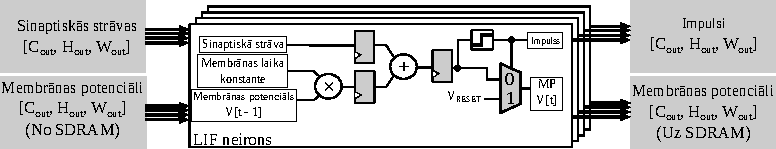
\includegraphics[width=\linewidth]{fig/lv/lif_neuron_core-v4.pdf}
  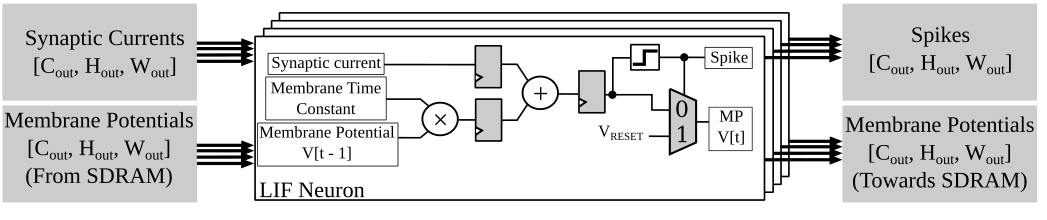
\includegraphics[width=\linewidth]{fig/lif_neuron_core-v4.png}
  \caption{LIF sliekšņa salīdzināšanas bloka aparatūras realizācija, kas atkārtota \(C_{out}\) reizes, ar membrānas potenciālu ārēju straumēšanu temporālai apstrādei ar stāvokļa saglabāšanu.}
  \label{fig:lif_arch}
\end{figure}

Vienu ieejas straumi izmanto sinaptiskajām strāvām \(X_o[t]\) no binārā telpiskā konvolūcijas filtra, savukārt otru straumi ārējai SDRAM atmiņai izmanto iepriekšējā laika soļa membrānas potenciālu \(V[t-1]\) ielādei un pašreizējo membrānas potenciālu \(V[t]\) ierakstīšanai atpakaļ. Abas straumes sinhronizē ar AXI-Stream sinhronizatoru, lai nodrošinātu pareizu laika saskaņojumu. Katrā slānī sliekšņa salīdzināšanas struktūra tiek atkārtota \(C_{out}\) reizes paralēlai apstrādei. Lai gan iepriekšējos darbos \cite{zhang2024, sommer2022} membrānas potenciāli tiek glabāti lokāli mikroshēmas iekšējā atmiņā tuvu apstrādes elementiem, lai samazinātu latentumu, BRAM izmantojums var strauji sasniegt pieejamo robežu, un risinājums slikti mērogojas līdz ar tīkla izmēru. Nepieciešamās atmiņas apjoms pieaug proporcionāli \(C_{out} \times H \times W\) un slāņu skaitam. Tādēļ piedāvātajā risinājumā mikroshēmas iekšējā BRAM glabā tikai konvolūcijas svarus, savukārt membrānas potenciāli tiek straumēti uz ārējo atmiņu un no tās.

Pēc membrānas integrēšanas un salīdzināšanas ar slieksni neirons ģenerē binārus izejas impulsus. Šos impulsus var novirzīt vai nu uz nākamo iekšējo slāni, vai uz AER kodētāja ieejas portu pārraidei kā ārējiem notikumiem.

Pēc izvēles ģenerētajām impulsu pazīmju kartēm var piemērot apvienošanas posmu, lai samazinātu to telpiskos izmērus. Apvienošanas slānis veic maksimuma apvienošanu konfigurējamā kodola logā ar programmējamu soli. Bināru impulsu reprezentācijām maksimuma apvienošana vienkāršojas līdz loģiskajai VAI operācijai pa elementiem apvienošanas logā. Tā kā bināru vērtību kopas maksimums ir viens ikreiz, kad logā ir aktīvs vismaz viens impulss, apvienošanas izeju var pierakstīt šādi:
\begin{equation}
  s_{\text{pool}} = \max(s_1, s_2, \ldots, s_n) = s_0 \vee s_1 \vee \ldots \vee s_n,
\end{equation}
kur \(\vee\) ir loģiskais VAI operators un \(n\) ir neironu skaits apvienošanas logā. Būtiski, ka apvienošanas bloku aparatūrā var realizēt ar vienkāršu kokveida VAI vārtu struktūru, izvairoties no aritmētiskām salīdzināšanas operācijām un saglabājot impulsu aktivitāti uztveres laukā. Šī operācija saglabā impulsu aktivitātes klātbūtni uztveres laukā, vienlaikus samazinot pazīmju karšu telpisko izšķirtspēju.


